\documentclass[11]{article}
\usepackage[utf8]{inputenc}

\usepackage{cite}
\usepackage{multicol}
\usepackage{float}
\usepackage{graphicx}
\usepackage[margin=1.25in]{geometry}
\usepackage{subcaption}
\author{Xavier Martín Ballesteros and Adrià Cabeza Sant'Anna \\ \small UNIVERSITAT POLITÈCNICA DE CATALUNYA}
\title{Flower detection using features\\ \large{Computer Vision, UPC}}
\date{\today}

\begin{document}
\maketitle
\vspace*{\fill}

\includegraphics[scale=0.4]{UPClogo.png}\par\vspace{1cm}

\newpage
\tableofcontents
\newpage 

\section{Introduction}
The aim of this assignment is to classify 12 different types of flowers using feature extraction. 
\begin{multicols}{3}
\begin{itemize}
\item BotodOr 
\item Crocus  
\item Fadrins   
\item Gerbera 
\item Hemerocallis 
\item Narcis
\item Buixol
\item DentdeLleo 
\item Fritillaria  
\item Girasol 
\item Lliri     
\item Viola

\end{itemize}
\end{multicols}

We have first implemented several ways to extract features that we believed could be key in order to classify correctly the flowers, we tested them, and using different classifiers (decisions trees, SVM or random forest) have tested the accuracy, specificity or sensitivity. 

\section{Descriptors}
In the following sections we will introduce different descriptors we have used to find those valuable features.

\subsection{Compactness}
After checking the different species of flowers we have to detect, one of the first descriptors we came up with was the \textbf{compactness}, the ratio of the perimeter to the area of the region. Since the shape and the size of each flower really varies, we think it can be a good discriminator. 
\medskip

To implement it we do need two things: \textbf{perimeter}(\textit{P}) and \textbf{area}(\textit{A}).

$$C= \frac{(P^2 / Area)} {4*\pi}$$
  \medskip
  
 To get the area we have used Matlab's \textbf{regionprops} utility, and to get the perimeter we have made \textbf{an erosion and a substraction}. 
 \medskip 
 
 \noindent In this example, we compare a \textit{} and a \textit{}.
 \begin{figure}[H]
    \begin{subfigure}[t]{.49\linewidth}
    \centering
  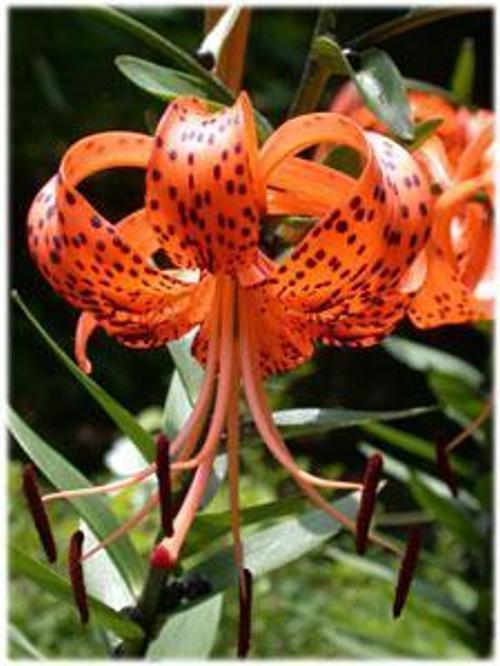
\includegraphics[scale=0.25]{images/compactness1.jpg}
  \caption{Compactness: \textbf{ }}
  \label{original}
    \end{subfigure}
    \begin{subfigure}[t]{.49\linewidth}
    \centering
    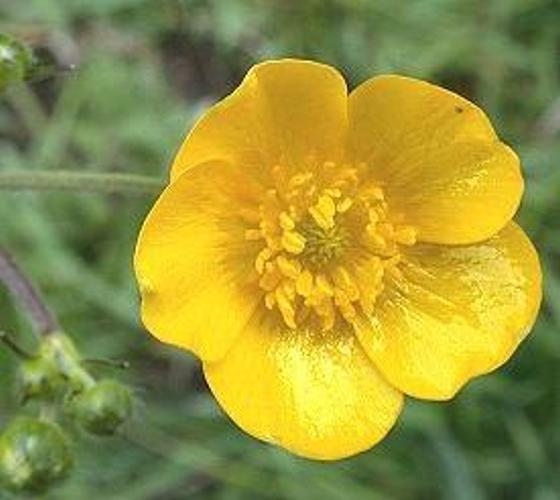
\includegraphics[scale=0.2]{images/compactness2.jpg}
    \caption{Compactness: \textbf{ }}
    \label{skez}
    \end{subfigure}
    \caption{Comparison of compactness}
\end{figure}


\subsection{Color Histogram}

\begin{figure}[H]
	\centering
	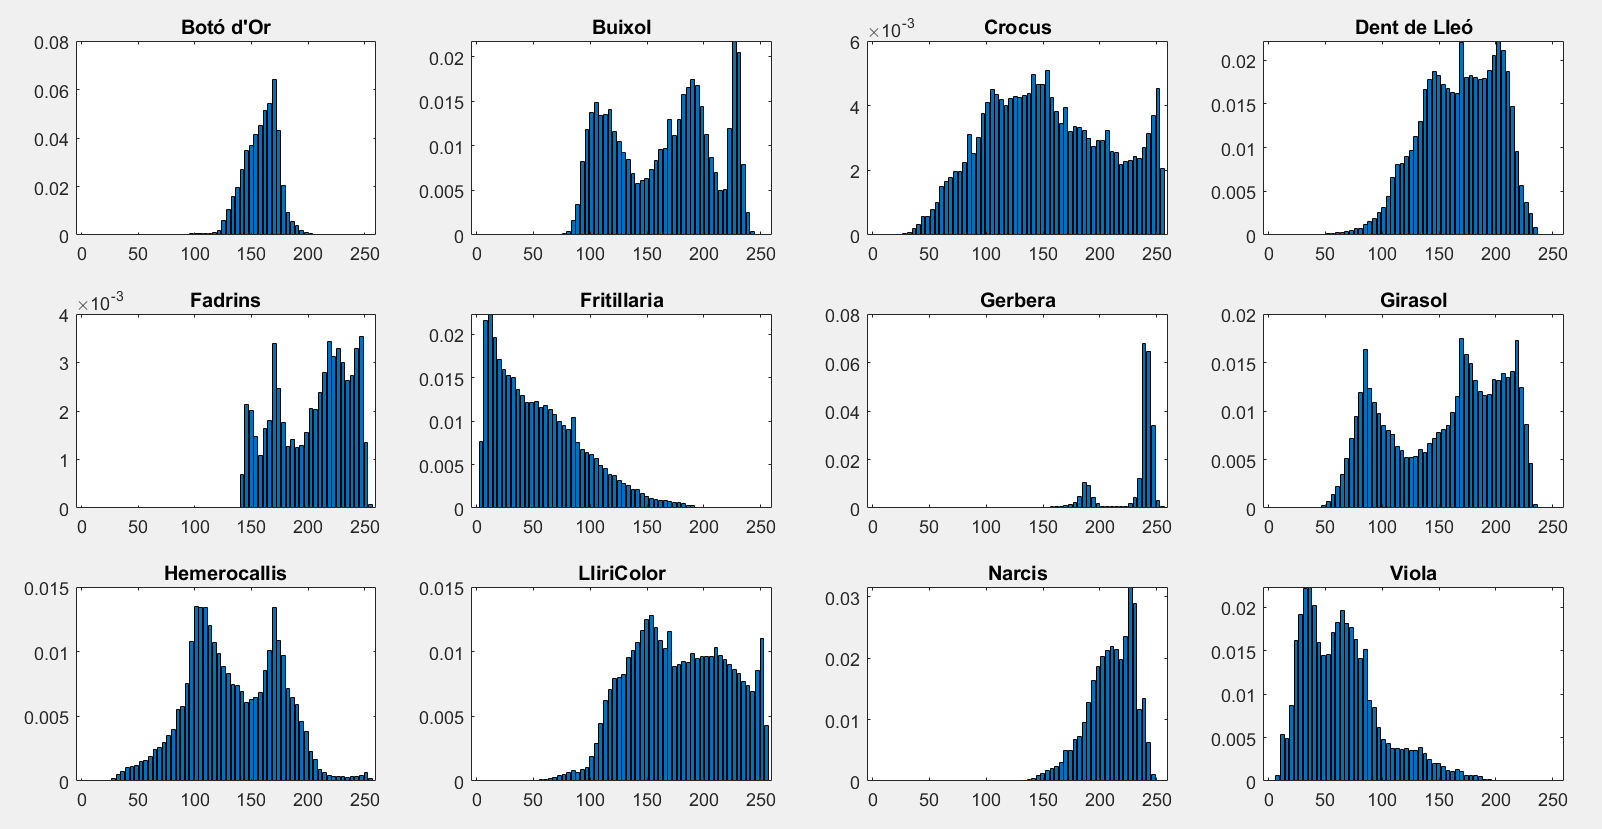
\includegraphics[scale=0.35]{images/colorHistogram1}
	\caption{Prova1.}
\end{figure}

\begin{figure}[H]
	\centering
	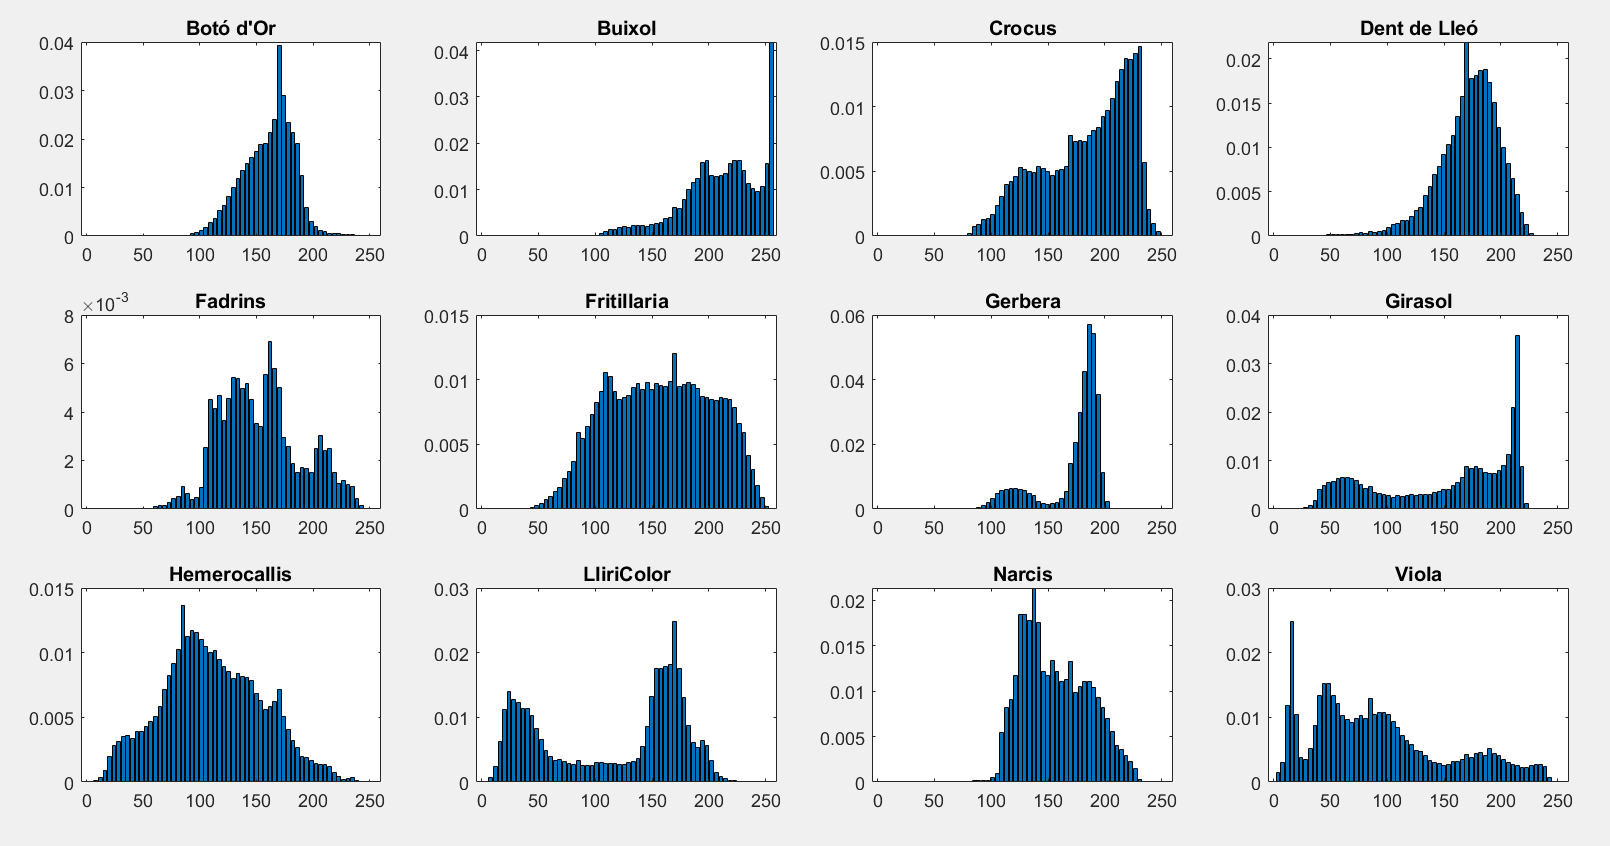
\includegraphics[scale=0.35]{images/colorHistogram2}
	\caption{Prova2.}
\end{figure}

\begin{figure}[H]
	\centering
	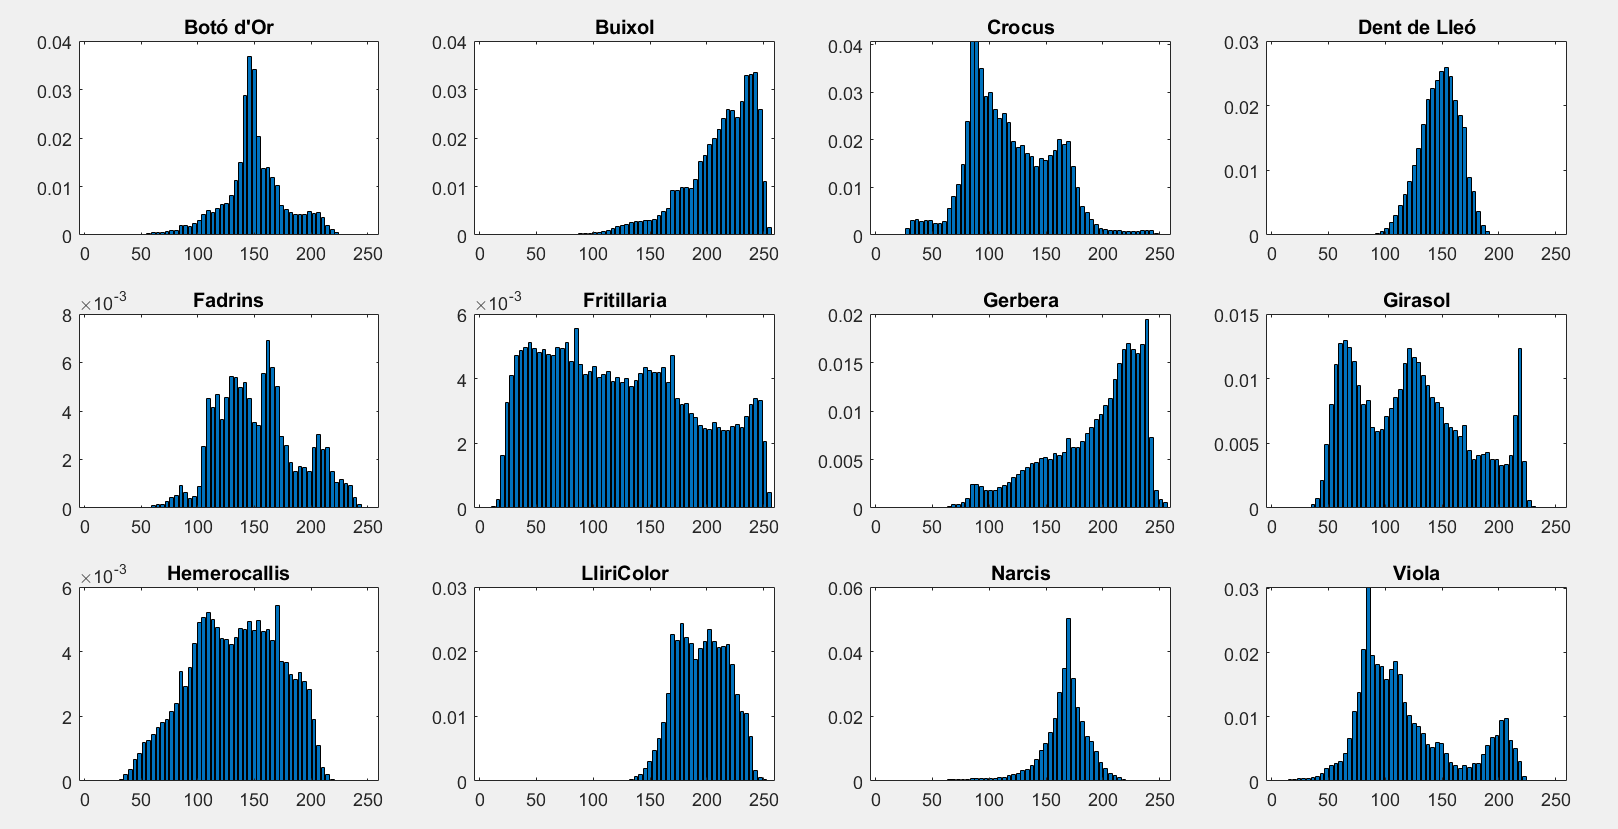
\includegraphics[scale=0.35]{images/colorHistogram3}
	\caption{Prova3.}
\end{figure}

\subsection{Number of petals}

This descriptor was one of the most difficult to think of. It can be done in several ways so we first had to choose in which way we wanted to attack the problem. In our case we decided to \textbf{skeletonize the flower}.
\medskip

To do so we used \textbf{bwmorph(image, 'skel', inf)} from Matlab. This	 creates the skeleton iterating as many times as necessary in order to not see any change between iterations (until it converges). Then we observed that sometimes the skeleton did not touch the contourn of the flower so we could not really count the petals; to solve it we applied an small erosion. The value of the disk structure was chosen based on several trials. 
\medskip

\noindent In this example using \textit{Boto d'Or} we get as a result 5 petals:
\begin{figure}[H]
    \begin{subfigure}[t]{.49\linewidth}
    \centering
  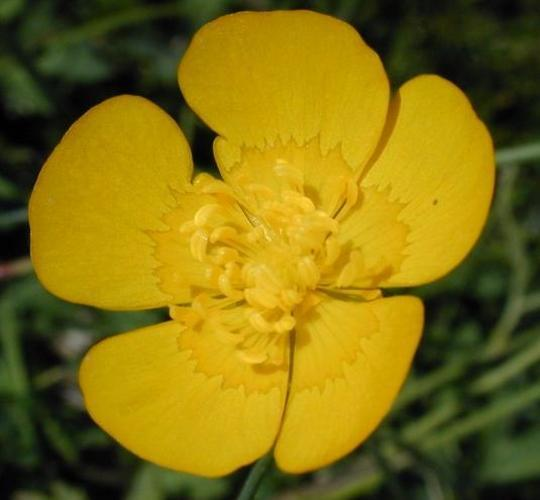
\includegraphics[scale=0.25]{images/numberOfPetalsOriginal.jpg}
  \caption{Original}
  \label{original}
    \end{subfigure}
    \begin{subfigure}[t]{.49\linewidth}
    \centering
    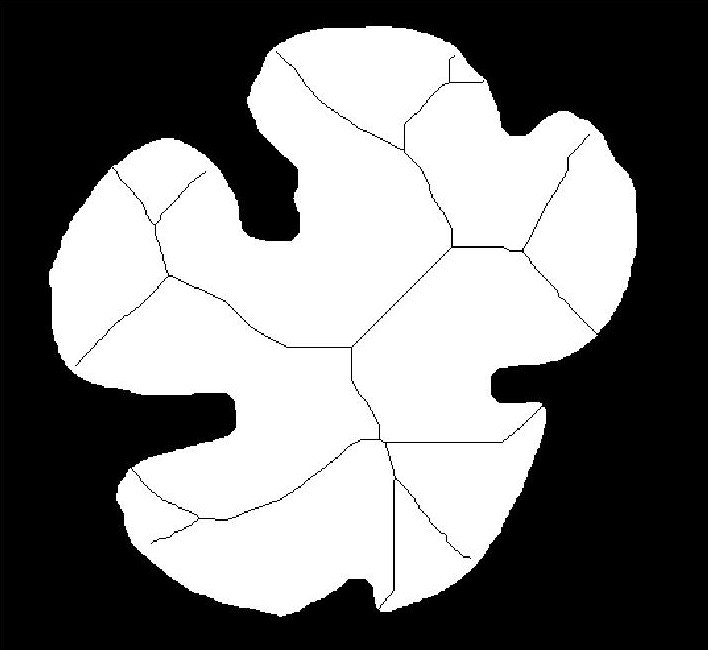
\includegraphics[scale=0.2]{images/numberOfPetals.jpg}
    \caption{Skez of the image}
    \label{skez}
    \end{subfigure}
\end{figure}


\subsection{Relative position of the centroid}

Just evaluating the position of the centroid would have been useless, it is not a feature of the flower per se. It can vary depending on the angle of the photo or the distance. However, if we calculate the relative position we can get really powerful information. 
\\

This two flowers, for example, should have really different values for this descriptor and it could be key in order to differenciate them in our classifier:
\begin{figure}[H]
    \begin{subfigure}[t]{0.45\textwidth}
    \centering
  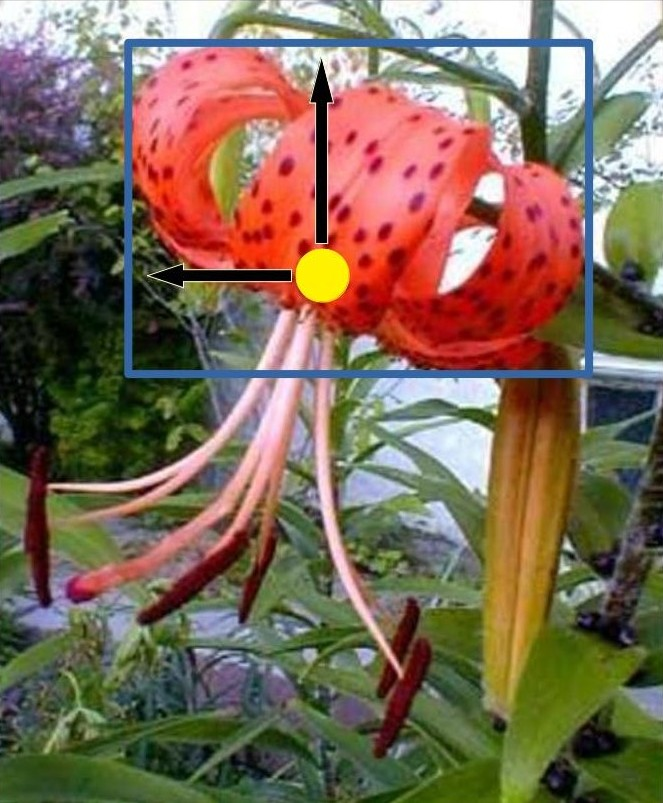
\includegraphics[scale=0.2]{images/hemerocallisCentroid.jpg}
    \caption{Centroid and bounding box of a \textit{Hemerocallis}}
    \label{centroidHemerocallis}
    \end{subfigure}
    \begin{subfigure}[t]{0.45\textwidth}
    \centering
    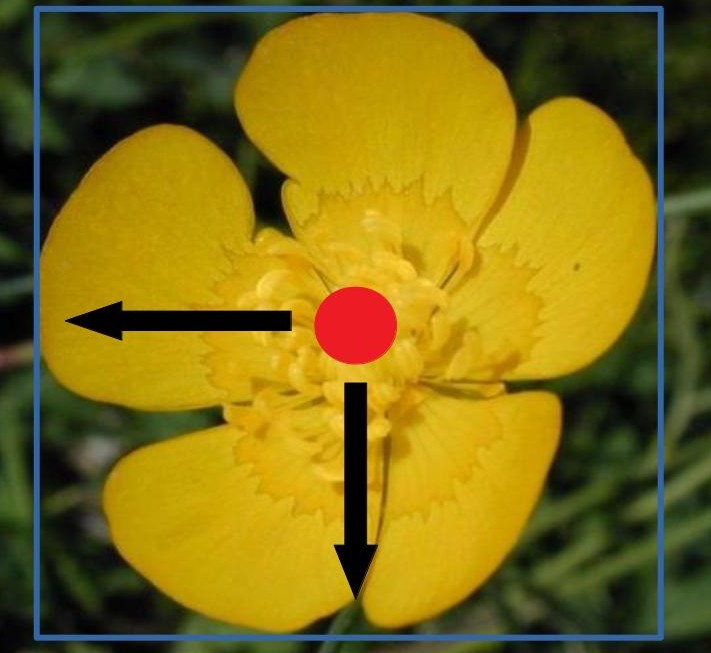
\includegraphics[scale=0.2]{images/GirasolCentroid.jpg}
    \caption{Centroid and bounding box of a \textit{Girasol}}
    \label{centroidgirasol}
    \end{subfigure}
\end{figure}

The way our descriptor is implemented is the following: we get the first and last pixels of X and Y axis in order to create the \textbf{bounding box}, then using \textbf{regions props} we get the \textbf{centroid of the flower} and finally we calculate the \textbf{relative position} of the centroid over the bounding box. 
\medskip

\begin{figure}[H]
	\centering
	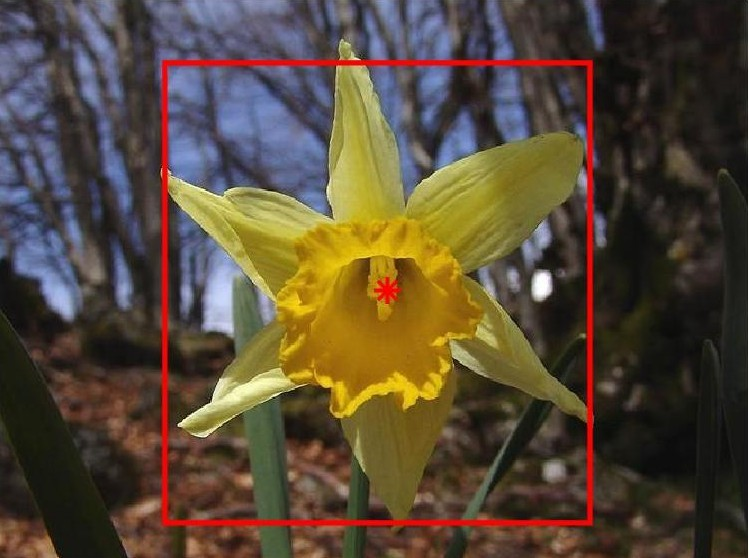
\includegraphics[scale=0.35]{images/centroid.jpg}
	\caption{Example of centroid and bounding box}
	\label{centroidNarcis}
\end{figure}


\subsection{Fourier descriptor: Shape}
It is known that we can use the Fourier transform to analyse and characterize the shape of a boundary. Since there are some flowers like the \textit{Hemerocallis} or the \textit{Girasol} that have a very specific shape; we believe that \textbf{the shape} can be a great descriptor. 

\begin{figure}[H]
    \begin{subfigure}[t]{0.45\textwidth}
    \centering
  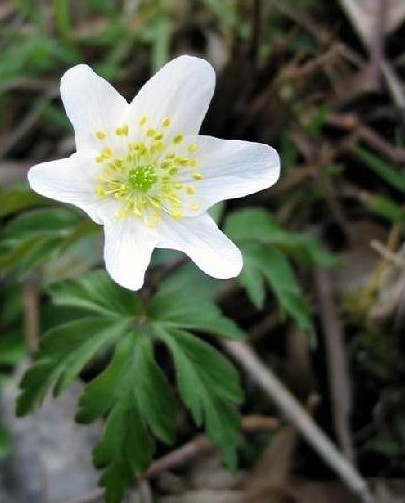
\includegraphics[scale=0.25]{images/originalfourier.jpg}
    \caption{Original}
    \label{originalfourier}
    \end{subfigure}
    \begin{subfigure}[t]{0.45\textwidth}
    \centering
    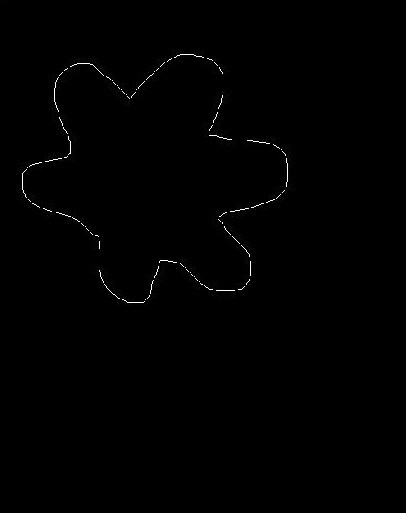
\includegraphics[scale=0.25]{images/shape.jpg}
    \caption{Shape}
    \label{fourier2}
    \end{subfigure}
    \label{fourier}
    \caption{Fourier descriptors}
\end{figure}


\subsection{Hogs form: Orientation}
Previously we have introduced a way to describe information about the shape. However, there are another ways to describe shapes. 
\\
As we wanted to have as proper features as possible, we have also implemented HOGs (histogram of oriented gradients), which basically describes \textbf{the shapes as the distribution of intensity gradient and edge directions}. To do it, we have used the utilities available at the \textit{Matlab Computer Vision Toolbox}.

\begin{figure}[H]
    \begin{subfigure}[t]{0.45\textwidth}
    \centering
  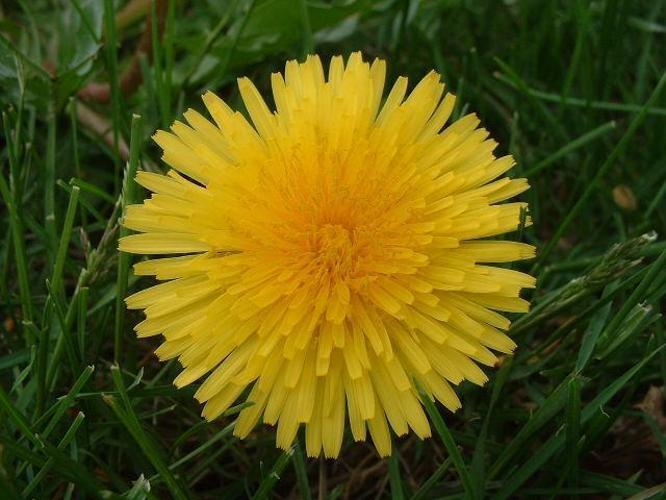
\includegraphics[scale=0.234]{images/originalhogg.jpg}
    \caption{Original}
    \label{originalhogg}
    \end{subfigure}
    \begin{subfigure}[t]{0.45\textwidth}
    \centering
    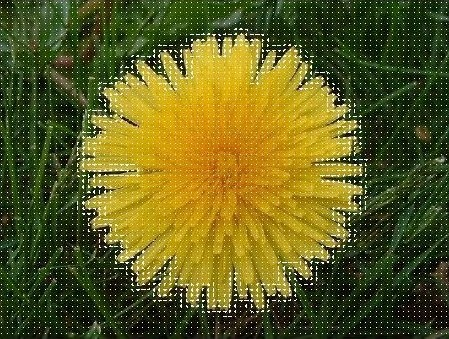
\includegraphics[scale=0.345]{images/hogg.jpg}
    \caption{Hog features}
    \label{hogg2}
    \end{subfigure}
    \label{hogg}
    \caption{HOG descriptors}
\end{figure}



\section{Classifiers}

\section{Experiments}
%NSE QUE FAREM AQUÍ PRO HO POSA A LO QUE HEM D'ENTREGAR

\section{The \textit{zero} class}

In order to increase the precision of our model, we have added a new class called \textit{zero}. This class represents all the flowers that are not from any of the 12 species that we are observing.
\medskip

To implement it we have written a script that \textbf{crawls google images and downloads photos of other species of flowers}. This will be very useful to create our dataset of \textit{zero} flowers. Morover, since these images are not segmented, we have looked for another source of flower pictures. In this case we have used \textbf{the Flowers Dataset from the Visual Geometry Group} (University of Oxford). This approach will help us to save time because we will have some flowers segmented by us (reviewed manually afterwards) and some already segmented (which we suppose are already correct).
\medskip

Our approach will consists in not training our classifier with that photos: we will assign a picture to that class if the confidence is less than a threshold. To test if actually works we will use the already mentioned test. 

Some of the flowers that can be seen in our \textit{zero} flower dataset are:
\begin{figure}[H]
    \begin{subfigure}[t]{0.45\textwidth}
    \centering
  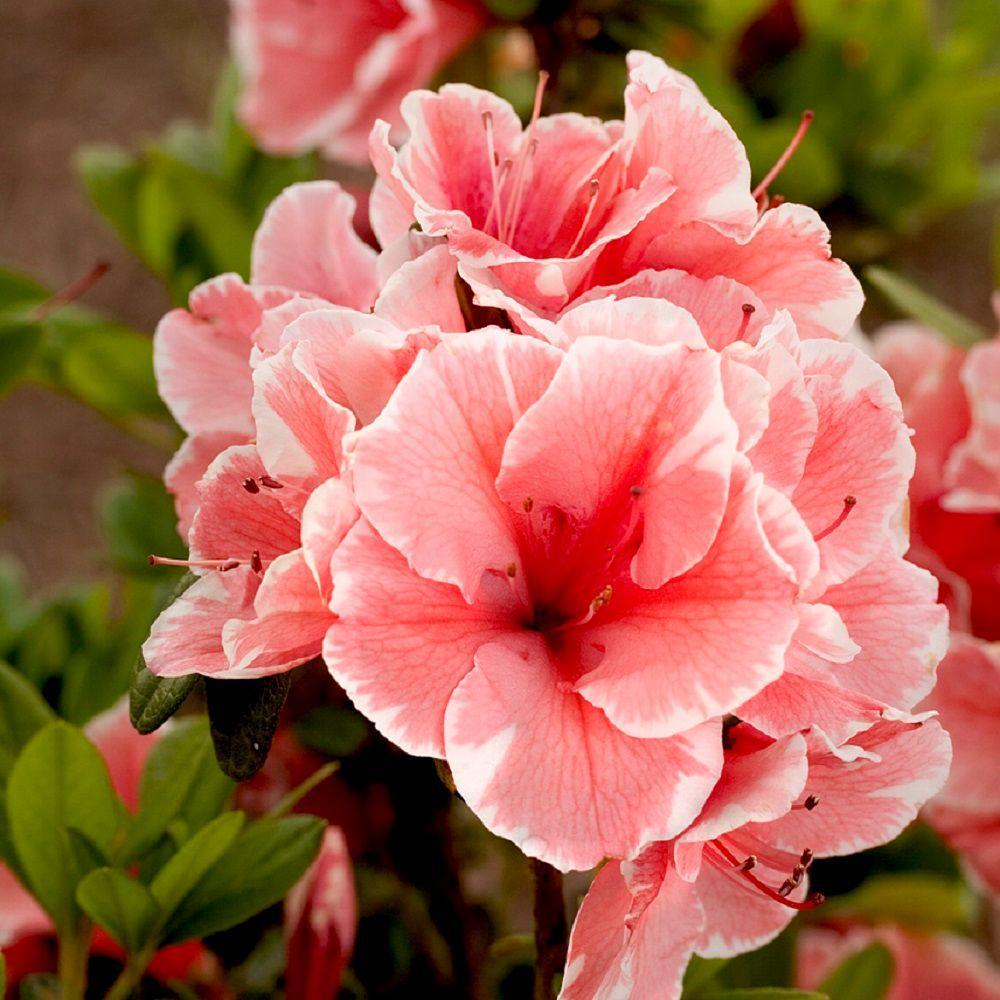
\includegraphics[scale=0.13]{images/azalea.jpg}
    \caption{Azalea}
    \label{azalea}
    \end{subfigure}
    \begin{subfigure}[t]{0.45\textwidth}
    \centering
    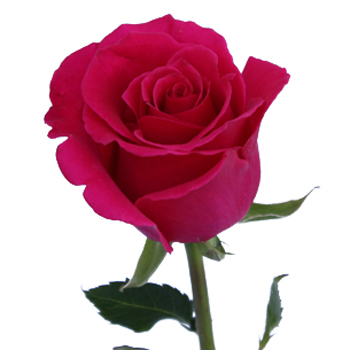
\includegraphics[scale=0.35]{images/roses.jpg}
    \caption{Roses}
    \label{roses}
    \end{subfigure}
\end{figure}

\begin{figure}[H]
    \begin{subfigure}[t]{0.45\textwidth}
    \centering
  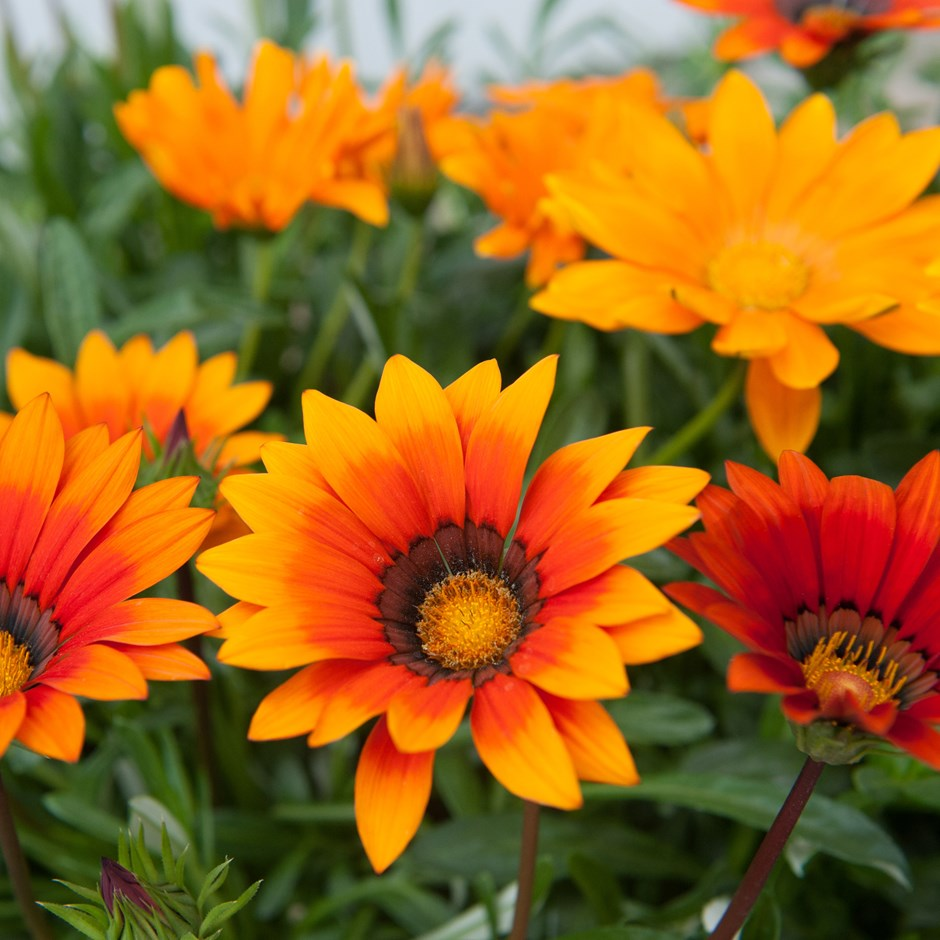
\includegraphics[scale=0.20]{images/gazania.jpg}
    \caption{Gazania}
    \label{gazania}
    \end{subfigure}
    \begin{subfigure}[t]{0.45\textwidth}
    \centering
    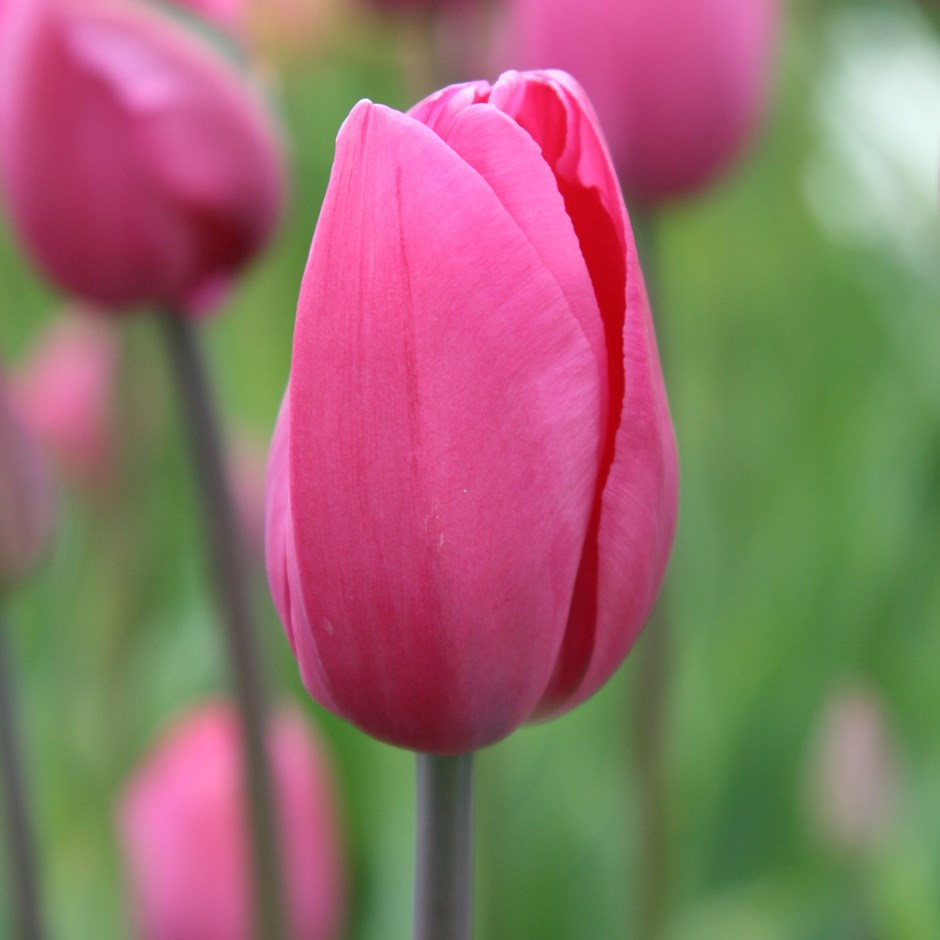
\includegraphics[scale=0.20]{images/tulip.jpg}
    \caption{tulip}
    \label{tulip}
    \end{subfigure}
    \label{zero}
    \caption{Zero class flowers}
\end{figure}


\section{Data augmentation}
In order \textbf{to strenghten our descriptors} we have also used the following public repository:  \textit{Albumentation: fast image augmentation library and easy to use wrapper around other libraries}(see more in References), which proporcionates facilities to augment the dataset including several transformations like: flipping, blurrring, RGB Shifting, Random contrast, Random brightness, etc...
\medskip

To decide which transformations we wanted to apply, we looked first to our descriptors and the importance of each feature. For example, we discarted the Channel Shuffle because we believe that the color is very important for our implementation. Then, based on trial and error, we picked some of them which gave us an overall better result. Finally we are using random variations of:
\begin{itemize}
    \item Brightness and Contrast
    \item Blur
    \item Rotations
    \item Flips
\end{itemize}
For example let's suppose that we are working with this \textit{Boto d'Or} image:
\begin{figure}[H]
    \centering
    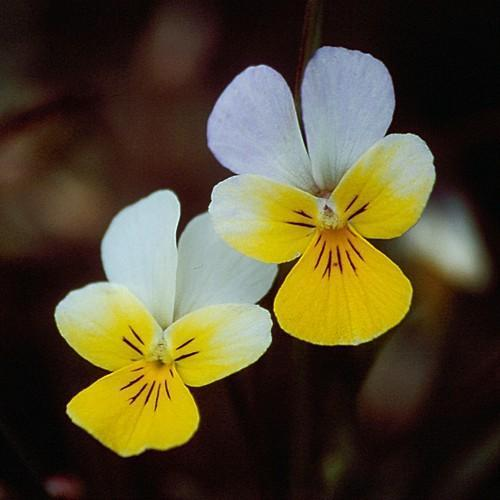
\includegraphics[scale=0.25]{images/original.jpg}
    \caption{Original picture}
    \label{original}
\end{figure}

The script we have implemented would apply the following transformations: 

\begin{figure}[H]
    \begin{subfigure}[t]{0.45\textwidth}
    \centering
  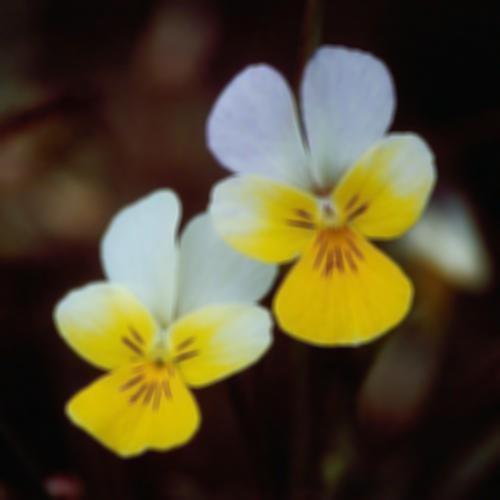
\includegraphics[scale=0.25]{images/blur.jpg}
    \caption{Blur transformation}
    \label{blur}
    \end{subfigure}
    \begin{subfigure}[t]{0.45\textwidth}
    \centering
    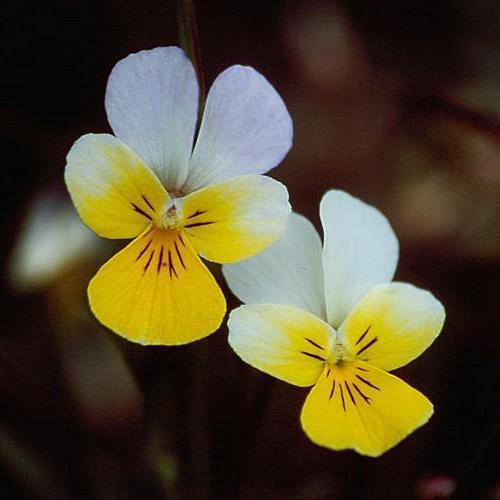
\includegraphics[scale=0.25]{images/horizontal.jpg}
    \caption{Horizontal Flip transformation}
    \label{horizontalflip}
    \end{subfigure}
\end{figure}

\begin{figure}[H]
    \begin{subfigure}[t]{0.45\textwidth}
    \centering
  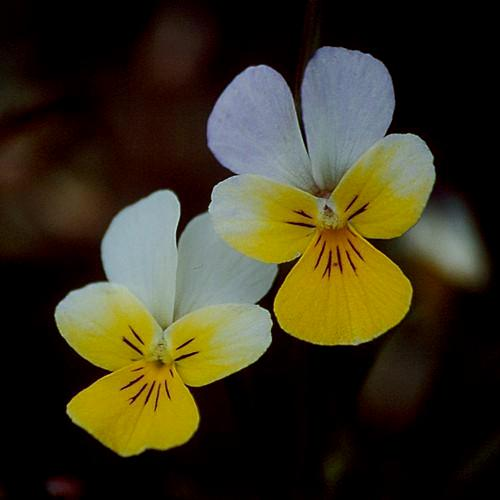
\includegraphics[scale=0.25]{images/brightness.jpg}
    \caption{Brightness and Contrast transformation}
    \label{brightness}
    \end{subfigure}
    \begin{subfigure}[t]{0.45\textwidth}
    \centering
    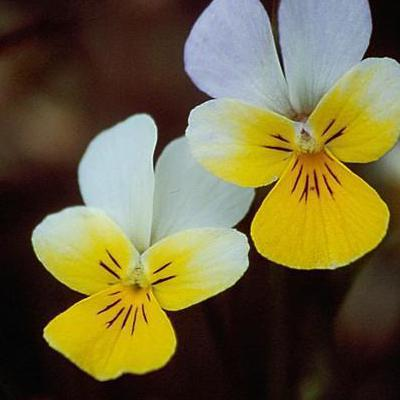
\includegraphics[scale=0.31]{images/scale.jpg}
    \caption{Scale transformation}
    \label{scale}
    \end{subfigure}
    \label{transformations}
    \caption{Data augmentation transformations}
\end{figure}

\section{Results}




\section{List of functions and libraries that have been used}
\begin{itemize}
\item \textbf{Bounding Box}: function that finds the relative position of the centroid from the bounding box. It uses the matlab utility \textbf{regionprops} to get the centroid.
\item \textbf{getCompactness}: function that calculates the compactness of a flower. It uses the matlab utility \textbf{regionprops} to get the area. To get the perimeter we have made an erosion and then a substraction. 
\item \textbf{getForma}: function that gets the shape Fourier descriptor. 
\item \textbf{getHog}: function that gets the HOG features. It uses the \textbf{Matlab Computer Vision Toolbox} utility \textbf{extractHOGFeatures}.
\item \textbf{getNumberPetals}: function that gets the number of petals using the skeleton. It uses the matlab utility \textbf{bwmorph} for the skeletonization. 
\item \textbf{histo3d}: function that gets the color information.
\item \textbf{Albumentations library}: for data augmentation issues.
\item \textbf{Google images download library}: to download several pictures of the \textit{zero} class.
\end{itemize}


\newpage
\begin{thebibliography}{100}
\bibitem{Image Segmentation}
\textit{Image Segmentation with MATLAB} [online]. Available at : https://www.mathworks.com/discovery/image-segmentation.html [Accessed 28 May 2019]


\bibitem{Flower dataset}
Nilsback, M-E. and Zisserman, A. (2008) \textit{Automated Flower Classification over a Large Number of Classes} [online] Available at:http://www.robots.ox.ac.uk/~vgg/publications/papers/nilsback08.pdf [Accessed 24 May 2019]


\bibitem{Albumentations}
    A. Buslaev (2018). Based on \textit{Albumentations: fast and flexible image augmentations} [online]. Paper available at:https://arxiv.org/abs/1809.06839. Code available at: https://github.com/albu/albumentations  [Accessed 3 June 2019].


\bibitem{Google images download}
    H. Vasa (2019). \textit{Python Script to download hundreds of images from 'Google Images'.} [online] Code available at: https://github.com/hardikvasa/google-images-download [Accessed 4 June 2019].



%%%%%%%%%%%%%%%%%%%%%%%%%%%%%%%%%%%%%%%%%%%%%%%%%%%%%%%%%%%%%%%%%%%%%%%%%%%%%%%%%%%%%%%
%\bibitem{Analysis of image Thresholding Methods for application to augmented reality enviornments}
%D. Martín Carabias (2012). \textit{Analysis of image Thresholding Methods for application to augmented reality enviornments.} [online] UCM. Available at: https://eprints.ucm.es/16932/1/Tesis\_Master\_Daniel\_Martin\_Carabias.pdf [Accessed 14 Mar. 2019].


%\bibitem{A survey of Thresholding Techniques}
%P. K. Sahoo, S. Soltani, K.C. Wong and Y.C. Chen (1988). \textit{A survey of Thresholding Techniques}. University of Waterloo, Waterloo, Canada  [Accessed 16 Mar. 2019].

%\bibitem{}N. Otsu, \textit{A Threshold Selection Method from Gray-Level Histograms}, in IEEE Transactions on Systems, Man, and Cybernetics, vol. 9, no. 1, pp. 62-66, Jan. 1979.
%[online] Available at http://ieeexplore.ieee.org/stamp/stamp.jsp?tp=\&arnumber=4310076\&is
%number=4310064 [Acessed 17 Mar. 2019].

%\bibitem{}Dr. Andrew Greensted (2010), \textit{Otsu Thresholding}. [online]. Available at http://www.labbookpages.co.uk/software/imgProc/otsuThreshold.html [Accessed 17 Mar. 2019].

%\bibitem{}Senthilkumaran,  N.  \&  Sivapriya,  M.  (2017),  \textit{Riddler's  Thresholding Algorithm  for  DNA  Image  Using  ISODATA  Modified  Algorithm} Journal  of Information Technology, Vol.3, No.2, pp.41-48. [online] Available at: http://www.ijitjournal.org/volume-3/issue-2/IJIT-V3I2P9.pdf [Accessed 17 Mar. 2019].

\end{thebibliography}

\end{document}
